\documentclass[10pt, a4paper]{article}
\usepackage[top=0.6in,bottom=1.0in,left=1.0in,right=1.0in]{geometry}
\usepackage{amsmath,amssymb}
\usepackage{hyperref}
\usepackage{graphicx,float,tikz}
\usepackage{listings}
\fontfamily{times}

\title{\large CS 4366: Senior Capstone Project \\ Dr. Sunho Lim \\ Project \#3 - Software Design Specification - Project Report \\ EmergenSeek}
\author{Suhas Bacchu \ Derek Fritz \ Kevon Manahan \ Annie Vo \ Simon Woldemichael}
\date{February 27, 2019}

\begin{document}

\maketitle
\vspace{-1cm}
\begin{abstract}
In this report, we describe and detail the layout and design of EmergenSeek. The structure of the system, at a high-level, consists of two components; a mobile client, developed using a Dart-based, cross-platform mobile framework called Flutter, and a backend Application Programming Interface (API), developed using Amazon Web Services, Google's Firebase platform, and the Go programming language. Each of these components is also broken down into their own modules and components. Respective design documentation, including UML class, use case, and sequence diagrams, are included as well.
\end{abstract}

\section{Project Restatement}
As a reminder, EmergenSeek is a mobile application which will provide users with multiuse, centralized emergency information and notification services. This application will provide friends and family members with priority connections in times of emergency or crisis. For the scope of the following two months, within this class, our main function requirements are as follows.
\begin{enumerate}
	\item[1.] S.O.S. button emergency broadcast --- The user shall be able to utilize the mobile client to press, (or press and hold) an S.O.S. button for automated notification of contacts and emergency services.
	\item[2.] Emergency service locator --- The user shall be able to utilize the mobile client to search for emergency service (i.e. hospitals, pharmacies, police boxes)
	\item[3.] Periodic notifications to contacts (location-based polling) --- The user shall be able to utilize the mobile client to send periodically send their location information to contacts.
	\item[4.] Granular permission definitions for contacts --- The user shall be given full control over what contacts receive what level of information.
	\item[5.] Lock screen display of health information for emergency services --- In the case of an S.O.S. situation, the user shall have their health information displayed for the convince of first responders.
\end{enumerate}

\section{Testbed}
\par ~ Before discussing the design documentation and the modular composition of the backend and frontend, we will describe how our project, both backend and frontend, will be tested and validated throughout development. At the core of our testbed is an Amazon Web Service known as CodeStar. CodeStar is comprised of four components; CodeCommit, CodeBuild, CodeDeploy, and CodePipeline. CodeCommit entails how the code and tooling of our project will be maintained. In this instance, we will be using two GitHub repositories, one for the backend and one for the frontend. Both are publicly available at \url{https://github.com/emergenseek}. 

\par ~ On every \texttt{git push} event (from a developers local machine to GitHub), CodeStar will begin a build sequence; this is where CodeBuild comes into play. CodeBuild will read a YAML specification \cite{two}, and per that specification, build our project. For our backend repository, the respective Go commands, will be invoked. This involves building all of our Lambda functions into statically linked binaries, testing them using our own custom unit tests, and preparing the static binaries for deployment by compressing them. Similarly, for the frontend, the respective Flutter commands will be invoked. This, again, involves unit and widget testing \cite{three} and building the Dart code into both an Android APK \cite{four} for distribution on the Google Play store and an iOS IPA for distribution on the Apple \footnote{Because distribution of apps to Apple's iOS App Store requires a developer partnership, which requires the payment of a fee, deployment of the iOS application is outside of the scope of this class} iOS App Store .

\par ~ Next, after the code has been tested and static binaries of both our Lambda functions and mobile clients have been built, they are deployed using both CodeDeploy and CodePipeline. CodeDeploy, intuitively, deploys our backend to Lambda (with API Gateway) and our mobile clients to their respective application stores (Google Play or Apple App). CodePipeline defines how they are deployed. The \emph{how} of the pipeline entails, more-so for the backend, what percentage of our newly deployed code should be accessed. CodePipeline is mainly used for defining different deployment stages (i.e. production, staging, or testing) and supports deployment patterns such as Canary or Blue/Green. Backing these services is an additional AWS service known as CloudFormation. CloudFormation provisions the necessary AWS resources, resource parameters, and their security policies, based on the contents of a second YAML definition.

\par ~ Lastly, on the backend side of things, because pushing our code and waiting for the entire deployment process before we can test our API is not a timely means of development, we will utilize Docker and Amazon's Serverless Application Model (SAM) \cite{five} to test on our local machines. Docker will replicate a Lambda environment within a local Docker machine (a Linux-based virtual machine running on a hypervisor) and allow us to invoke the function using a \texttt{localhost} endpoint.

\newpage

\section{Design Documentation}
\par ~ In this section, we will discuss the various details of our design documents. In each subsection below, diagrams are displayed and followed by a brief description of each of the components within the associated diagram.

\subsection{UML Class Diagram}
In this subsection, we will display and briefly explain class diagrams relevant to our application.
\subsubsection{Backend}
\begin{figure}[H]
  \centerline{
  	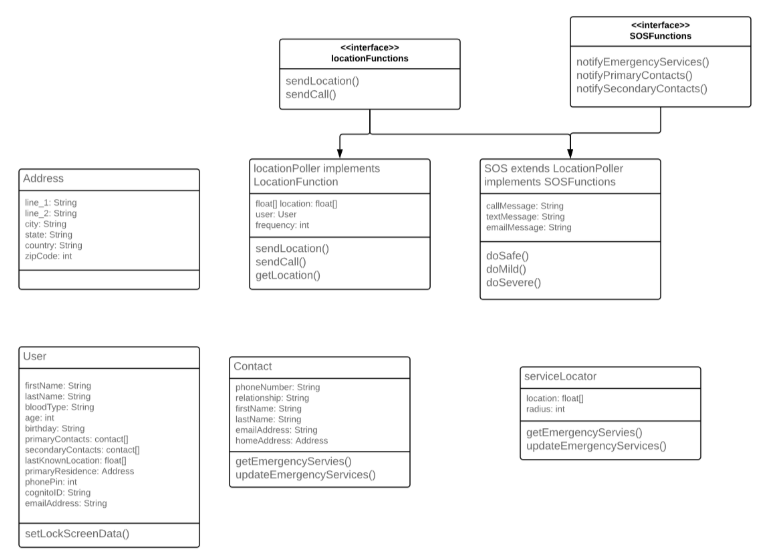
\includegraphics[scale=1.3]{diagrams/backend-class.png}
  }  
  \caption{Class diagram for the backend.}
\end{figure}

\begin{enumerate}
\item[1.] Address --- Encapsulates the data necessary for representing an address.
\item[2.] User --- Encapsulates the data necessary for representing a user. Has 1 method which retrieves the user's information using a Lambda function for display on the lock screen.
\item[3.] Contact --- Encapsulates the data necessary for representing a user's contact. Has 2 methods which get and update the contact on the emergency services map so that the user may see which of their contacts are nearby.
\item[4.] ServiceLocator --- Encapsulates the data necessary for performing location based functions. Has two methods which will get and update emergency service locations for the map on the client.
\item[5] LocationFunctions --- (Interface) This interface contains the polymorphic methods necessary for performing location related functions. This interface is implemented by the LocationPoller instance.
\item[6.] SOSFunctions --- (Interface) This interface contains the polymorphic methods necessary for providing functionality to the S.O.S. button. This interface is implmeneted by the SOS instance.
\item[7.] LocationPoller --- Encapsulates the data necessary for providing functionality to the location polling feature. This instance implements the LocationFunctions interface.
\item[8.] SOS --- Encapsulates the data necessary for defining the SOS buttons functionality. This instance inherits the LocationPoller instance and implements the SOSFunctions interface. It should be noted that while the \texttt{emailMessage} attribute does exist, for the scope of this class, we will focus on SMS and voice.
\end{enumerate}

\subsubsection{Frontend}
\begin{figure}[H]
  \centerline{
  	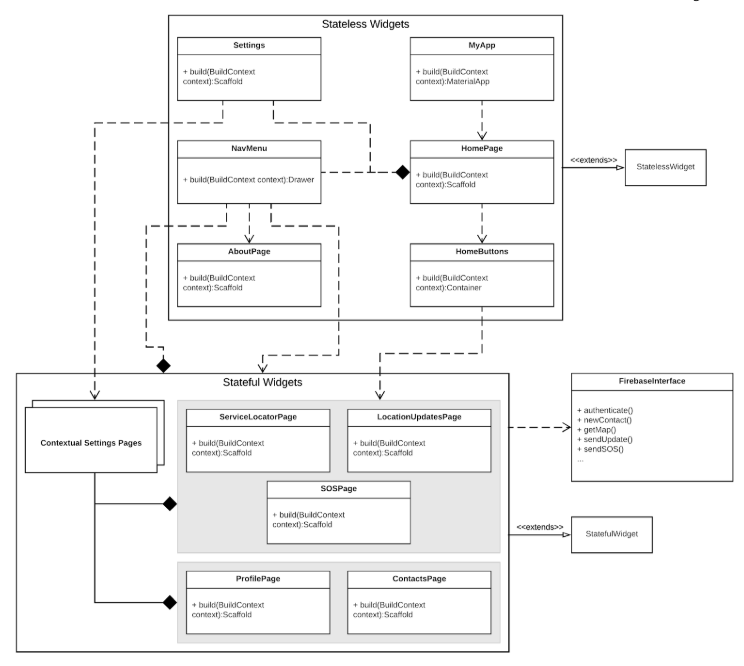
\includegraphics[scale=1.3]{diagrams/client-class-1.png}
  }  
  \caption{Full client class diagram for the Flutter code base. The top half defines a group of stateless widgets and the botom half defines a group fo stateful widgets. The largest difference between the two is, stateful widgets are responsible for dynamically changing based on the current \emph{state} of the application. For example, when the user logs in, the application should contain all of the user's information without having to prompt the user for that information repeatedly. In Flutter, all user interface components are widgets. Widgets are either stateful or stateless. NUniversal components such as NavMenu and Settings act as widgets within others. This can be related to component inheritance. Notice The \texttt{build} method in every components defines how the component is rendered, what data it is responsible for encapsulating, and the logic necessary for invoking interactions with the backend API.}
\end{figure}


\subsection{UML Use Case Diagram}
In this subsection, we will display and briefly explain use case diagrams relevant to our application.
\begin{figure}[H]
  \centerline{
  	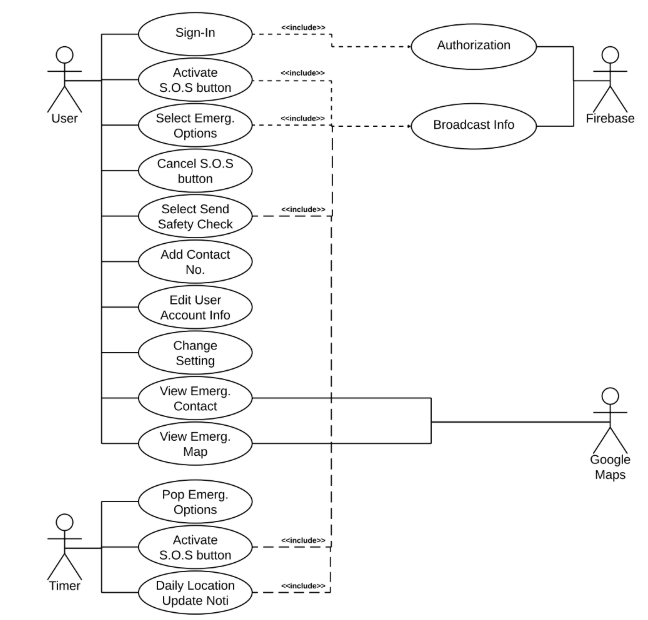
\includegraphics[scale=.8]{diagrams/use-case.png}
  }  
  \caption{Use-case Diagrams for Emegenseek}
\end{figure}

\par ~ Below is an enumeration of each of the use case objects with respect to the \emph{User}, their inclusions, and their involved actors. It should be noted that these use case inclusions are very high level, taking into consideration scope and constraints, and should be treated as such.

\begin{enumerate}
	\item[1.] Sign-in: The user shall be able to sign-in to the system, dependent on the authorization functionality of Firebase (actor).
	\item[2.] Activate S.O.S. button: The user shall be able to activate the S.O.S. button with full functionality, dependent on a timer actor which will ensure that no false positives are triggered.
	\item[3.] Select Emergency Options: The user shall be able to select emergency options and resources, dependent on our backend to retrieve this map information. A timer actor is responsible for how the system will updated 
	\item[4.] Cancel S.O.S. button: The user shall be able to dismiss an accidentally or unwanted trigger of the S.O.S. button.
	\item[5.] Select Send Safety Check: The user shall be able to send safety check-in messages, dependent on a timer which may automatically send these messages on behalf of the user
	\item[6.] Add Contact Number: The user, utilizing native mobile features, shall be able to add their personal contacts to the application.
	\item[7.] Edit User Account Info: The user shall be able to edit their account information for the purpose of keeping all content, health and person, relevant and up to date.
	\item[8.] Change Setting: The user shall be able to change their application setting per their liking. This includes being able to update message frequencies and contact permissions.
	\item[9.] View Emergency Contact: The user shall be able to view their contacts, nearby or otherwise, on a map; dependent on Google's Geocoding API for well defined location information.
	\item[10.] View Emergency Map: The user shall be able to view a map containing emergency services available within a specified radius; dependent on Google Maps for location search results. 
\end{enumerate}

\subsection{UML Sequence Diagrams}
In this subsection, we will display and briefly explain sequence diagrams relevant to our application.

\begin{figure}[H]
  \centerline{
  	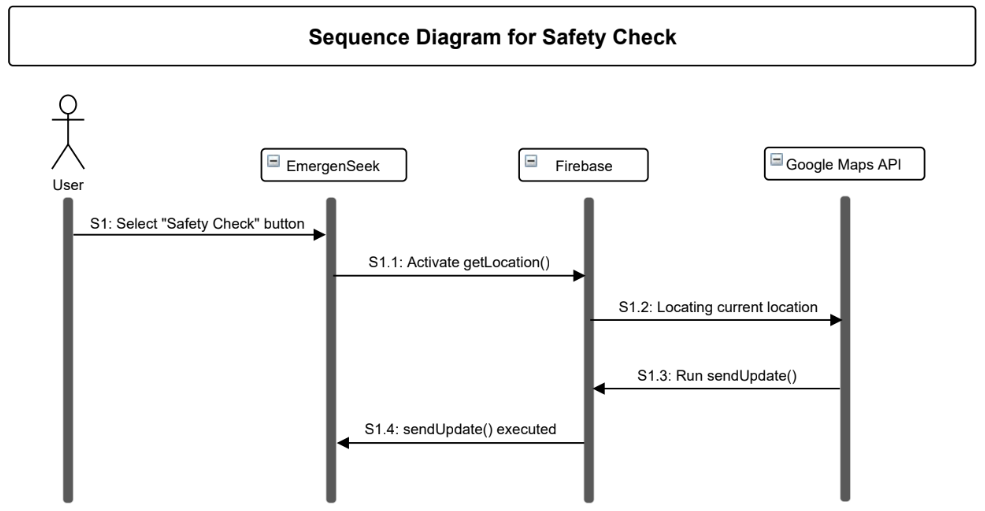
\includegraphics[scale=0.8]{diagrams/sequence-1.png}
  }  
  \caption{In this sequence diagram, we describe the interactions involved for performing a safety check. Activating the safety check-in feature will send an instant location-based update. This feature will request location polling from the backend. The client will receive confirmation of the update.}
\end{figure}

\begin{figure}[H]
  \centerline{
  	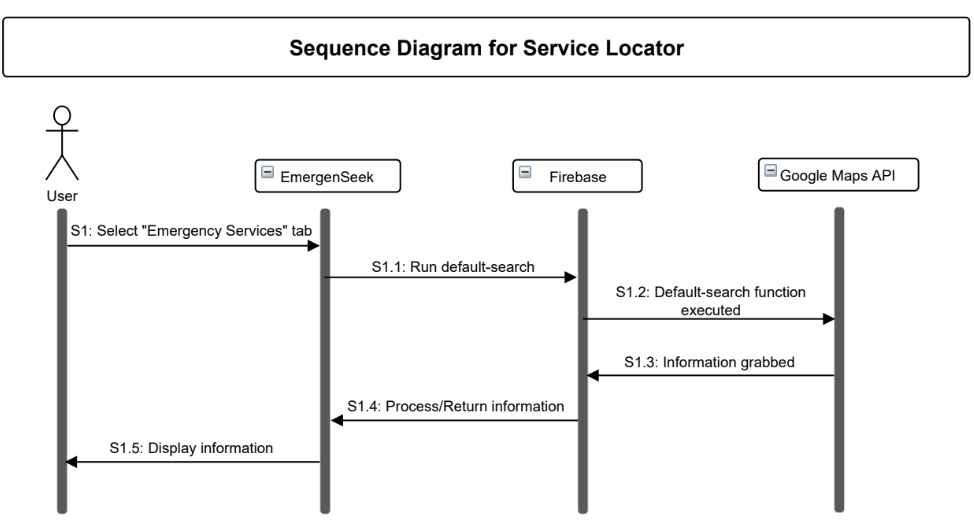
\includegraphics[scale=0.8]{diagrams/sequence-2.png}
  }  
  \caption{In this sequence diagram, we describe the interactions involved for using the service locator. Default search criteria will be used upon opening locator. Search request will be routed to backend and set to the API. Response info is then routed back to the client.}
\end{figure}

\begin{figure}[H]
  \centerline{
  	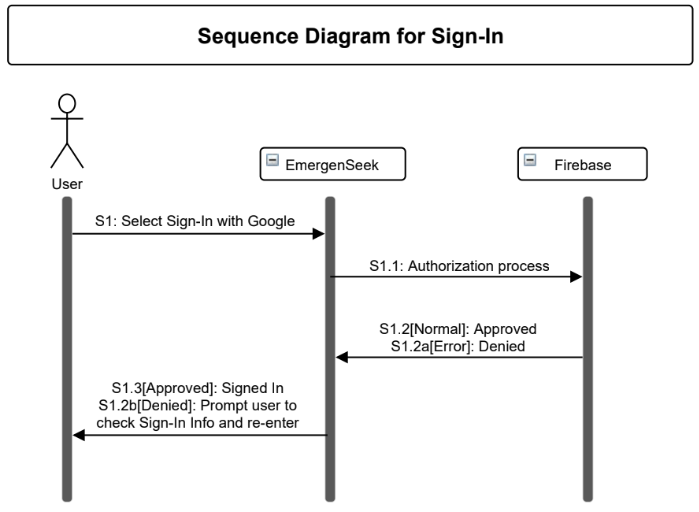
\includegraphics[scale=0.8]{diagrams/sequence-3.png}
  }  
  \caption{In this sequence diagram, we describe the interactions involved for signing a user in. User sign-in process handled via Firebase authentication. The result of Firebase request is returned to the client.}
\end{figure}

%
%\begin{figure}[H]
%  \centerline{
%  	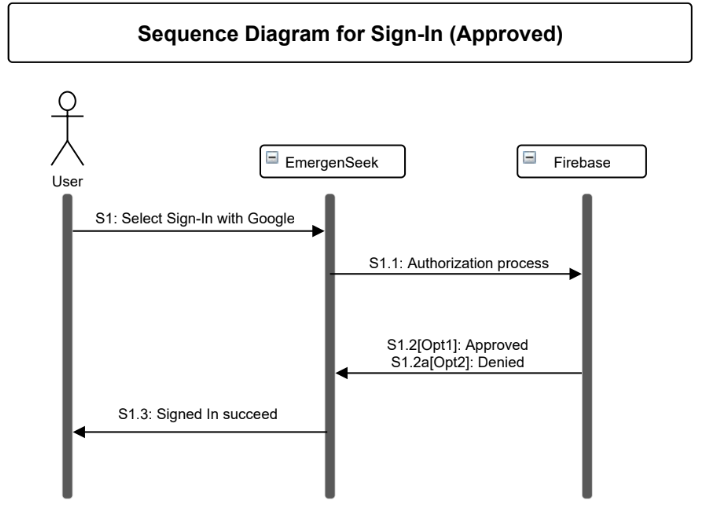
\includegraphics[scale=0.6]{diagrams/sequence-4a.png}
%  	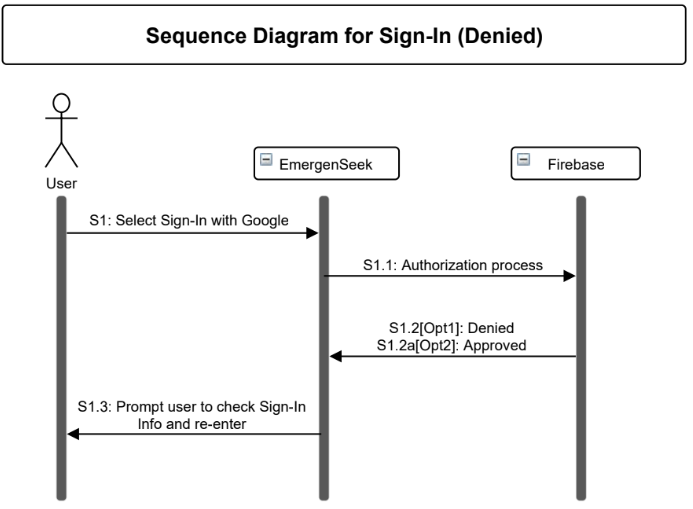
\includegraphics[scale=0.6]{diagrams/sequence-4b.png}
%  }  
%  \caption{In these sequence diagrams,}
%\end{figure}
%

\begin{figure}[H]
  \centerline{
  	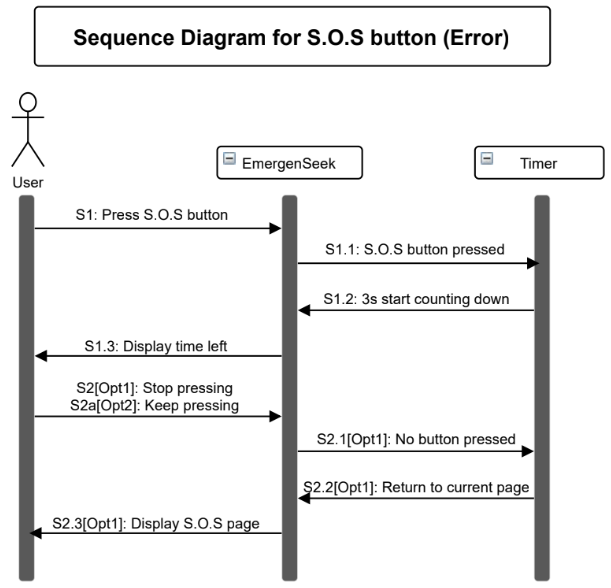
\includegraphics[scale=0.6]{diagrams/sequence-5a.png}
  	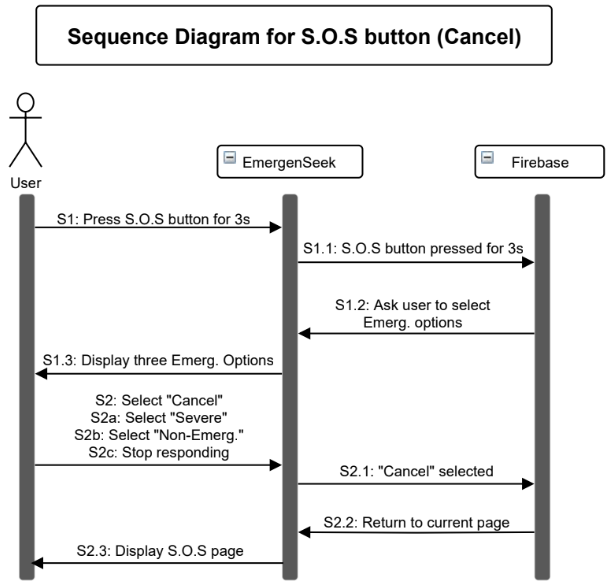
\includegraphics[scale=0.6]{diagrams/sequence-5b.png}
  } 
  \centerline{
  	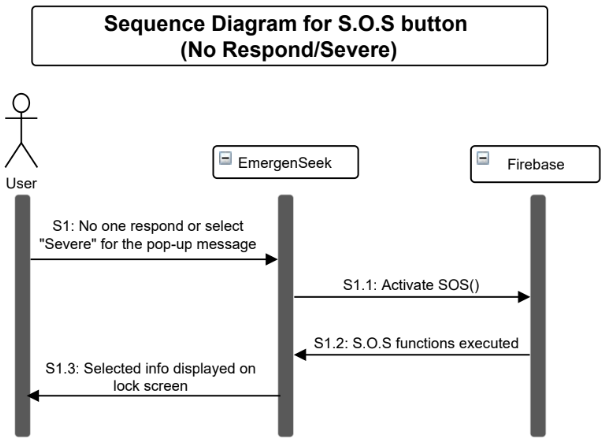
\includegraphics[scale=0.6]{diagrams/sequence-5c.png}
  	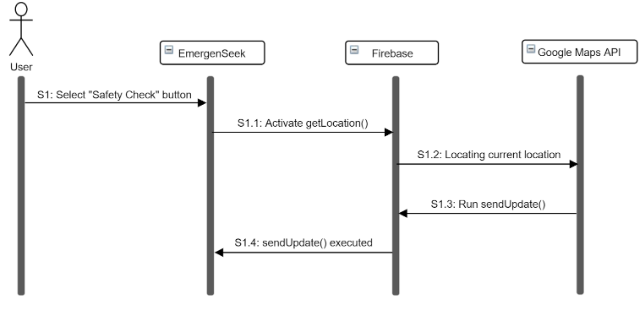
\includegraphics[scale=0.7]{diagrams/sequence-5d.png}
   } 
  \caption{In these sequence diagrams, we enumerate the different possibilities for the user interacting with the S.O.S. button. \emph{Top left}: False S.O.S. activation is countered by monitoring for a 3 second press-and-hold. If user fails to carry out the activation, the S.O.S. button will return to its inactive state. \emph{Top right}: After activating the S.O.S. button, a selection + confirmation prompt will appear. Here, users may opt to cancel the S.O.S. alert. \emph{Bottom left}: S.O.S. alert will default to severe if user is unable to confirm. This function involves the inclusion of the following functions getContacts(), getLocation(), sendSMS(), sendVoiceCall(), displayInfo(). \emph{Bottom Right}: Activating the safety check-in feature will send an instant location-based update. The client will receiv confirmation of the update. This option is simply for users to notify their contacts in a non-emergency event.}
\end{figure}

\newpage

\section{Client Mockups}
\par ~ In this section, we will enumerate some low and high fidelity mockups for the frontend.


\begin{figure}[H]
\minipage{0.32\textwidth}
  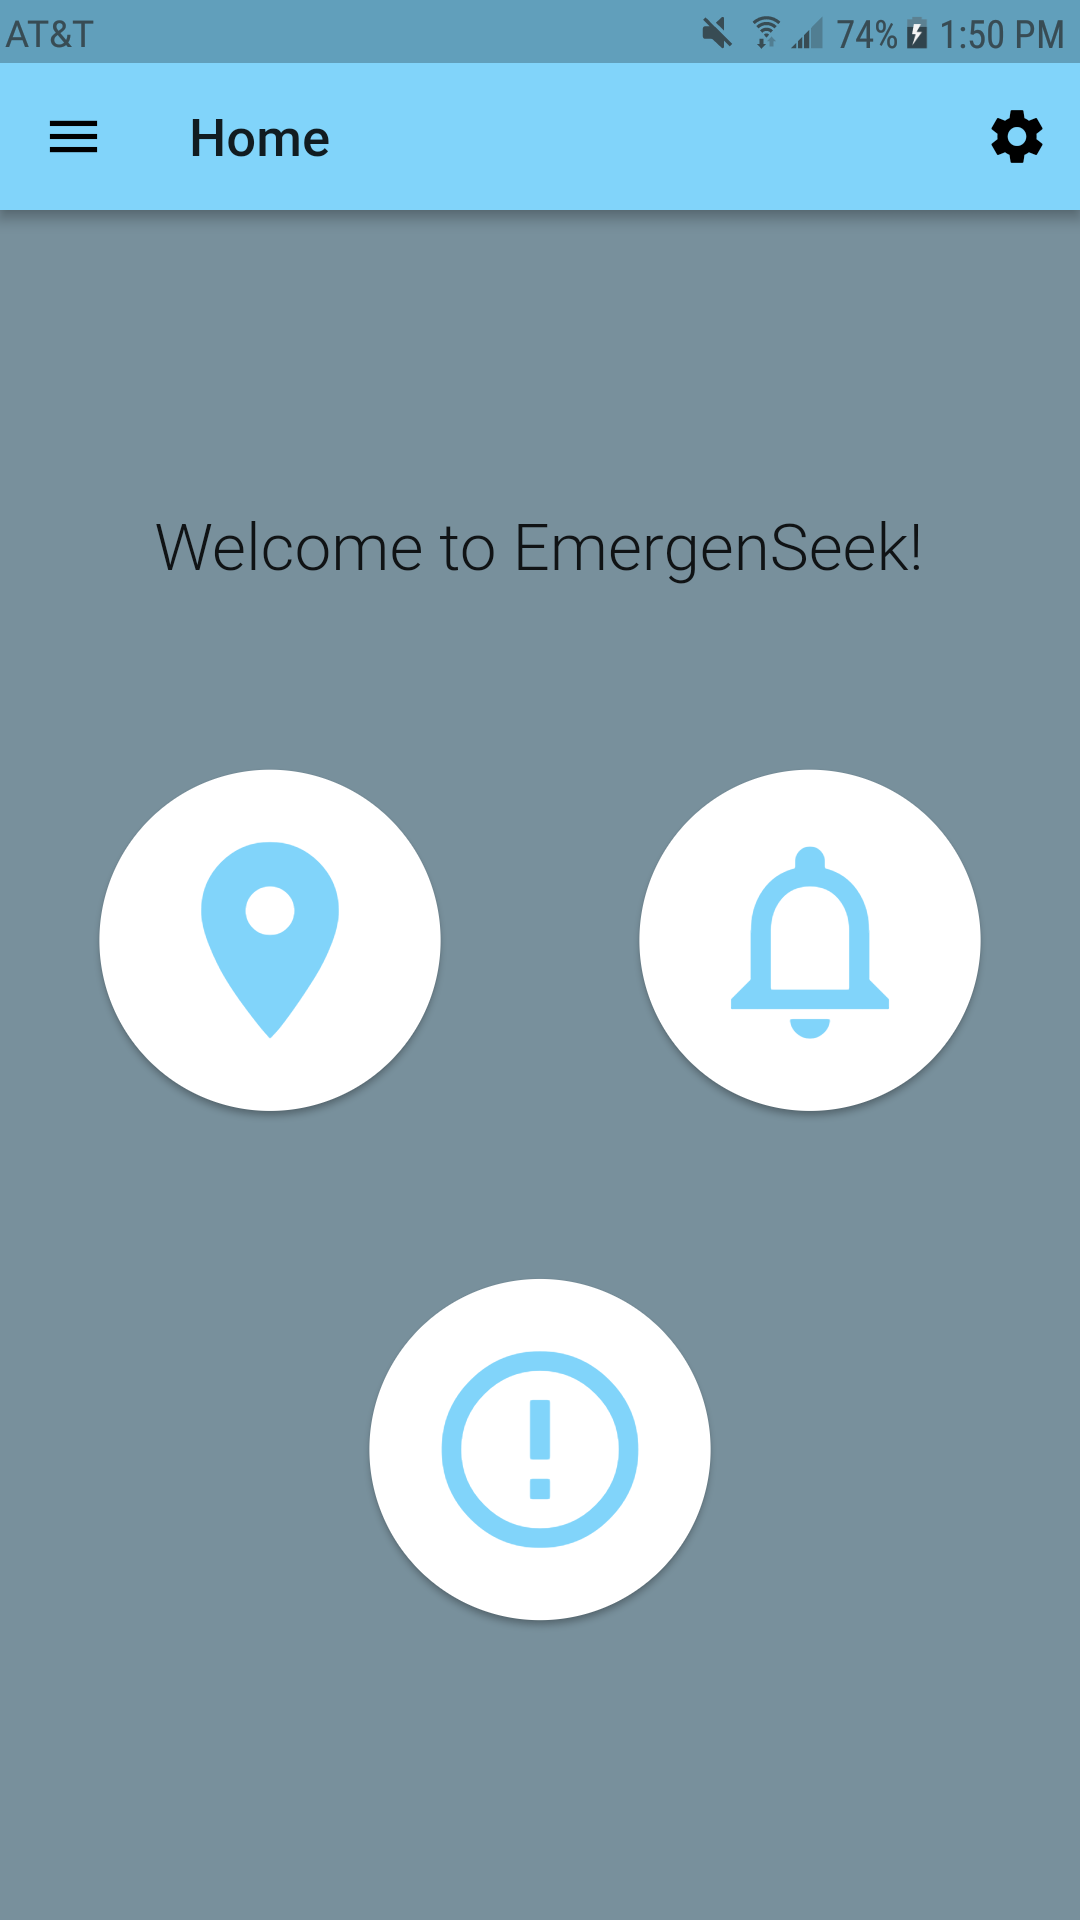
\includegraphics[width=\linewidth]{demo_home.png}
  \caption{High-fidelity, implemented, screenshot of the mobile client's home page.}\label{fig:mobile1}
\endminipage\hfill
\minipage{0.32\textwidth}
  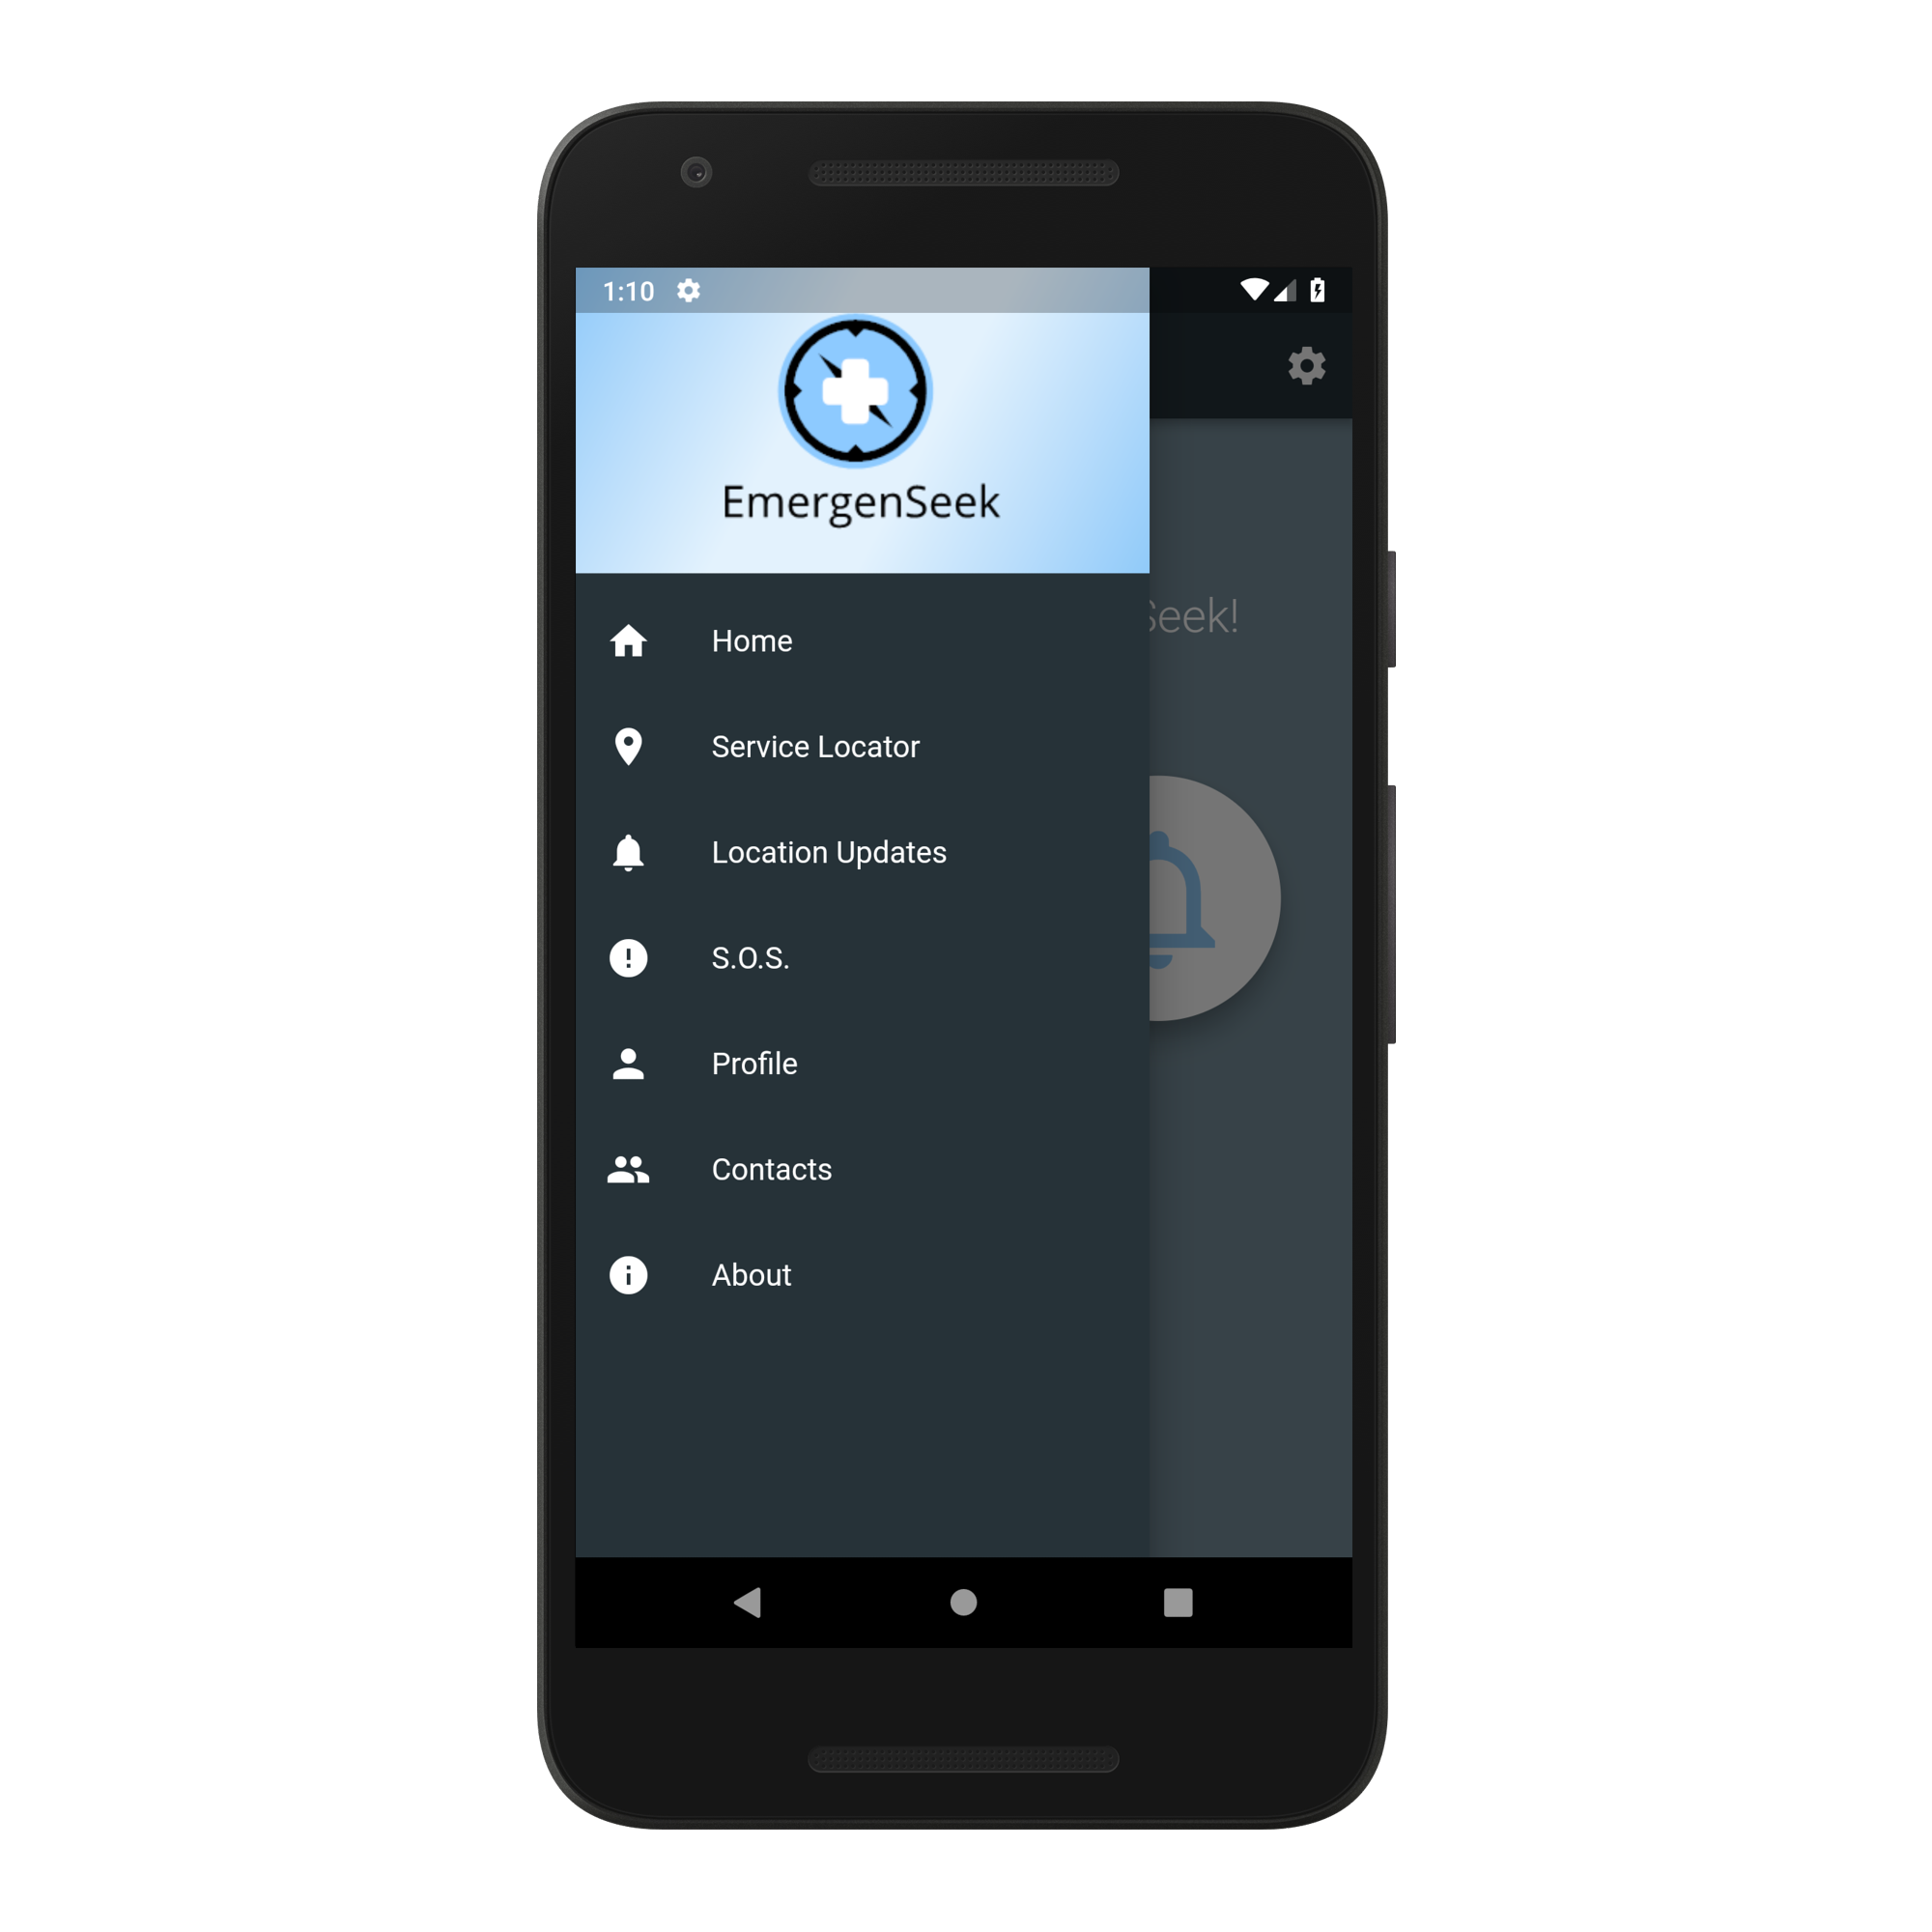
\includegraphics[width=\linewidth]{demo_navmenu.png}
  \caption{High fidelity, implemented, screenshot of the mobile client's navigation menu.}\label{fig:mobile2}
\endminipage\hfill
\minipage{0.32\textwidth}%
  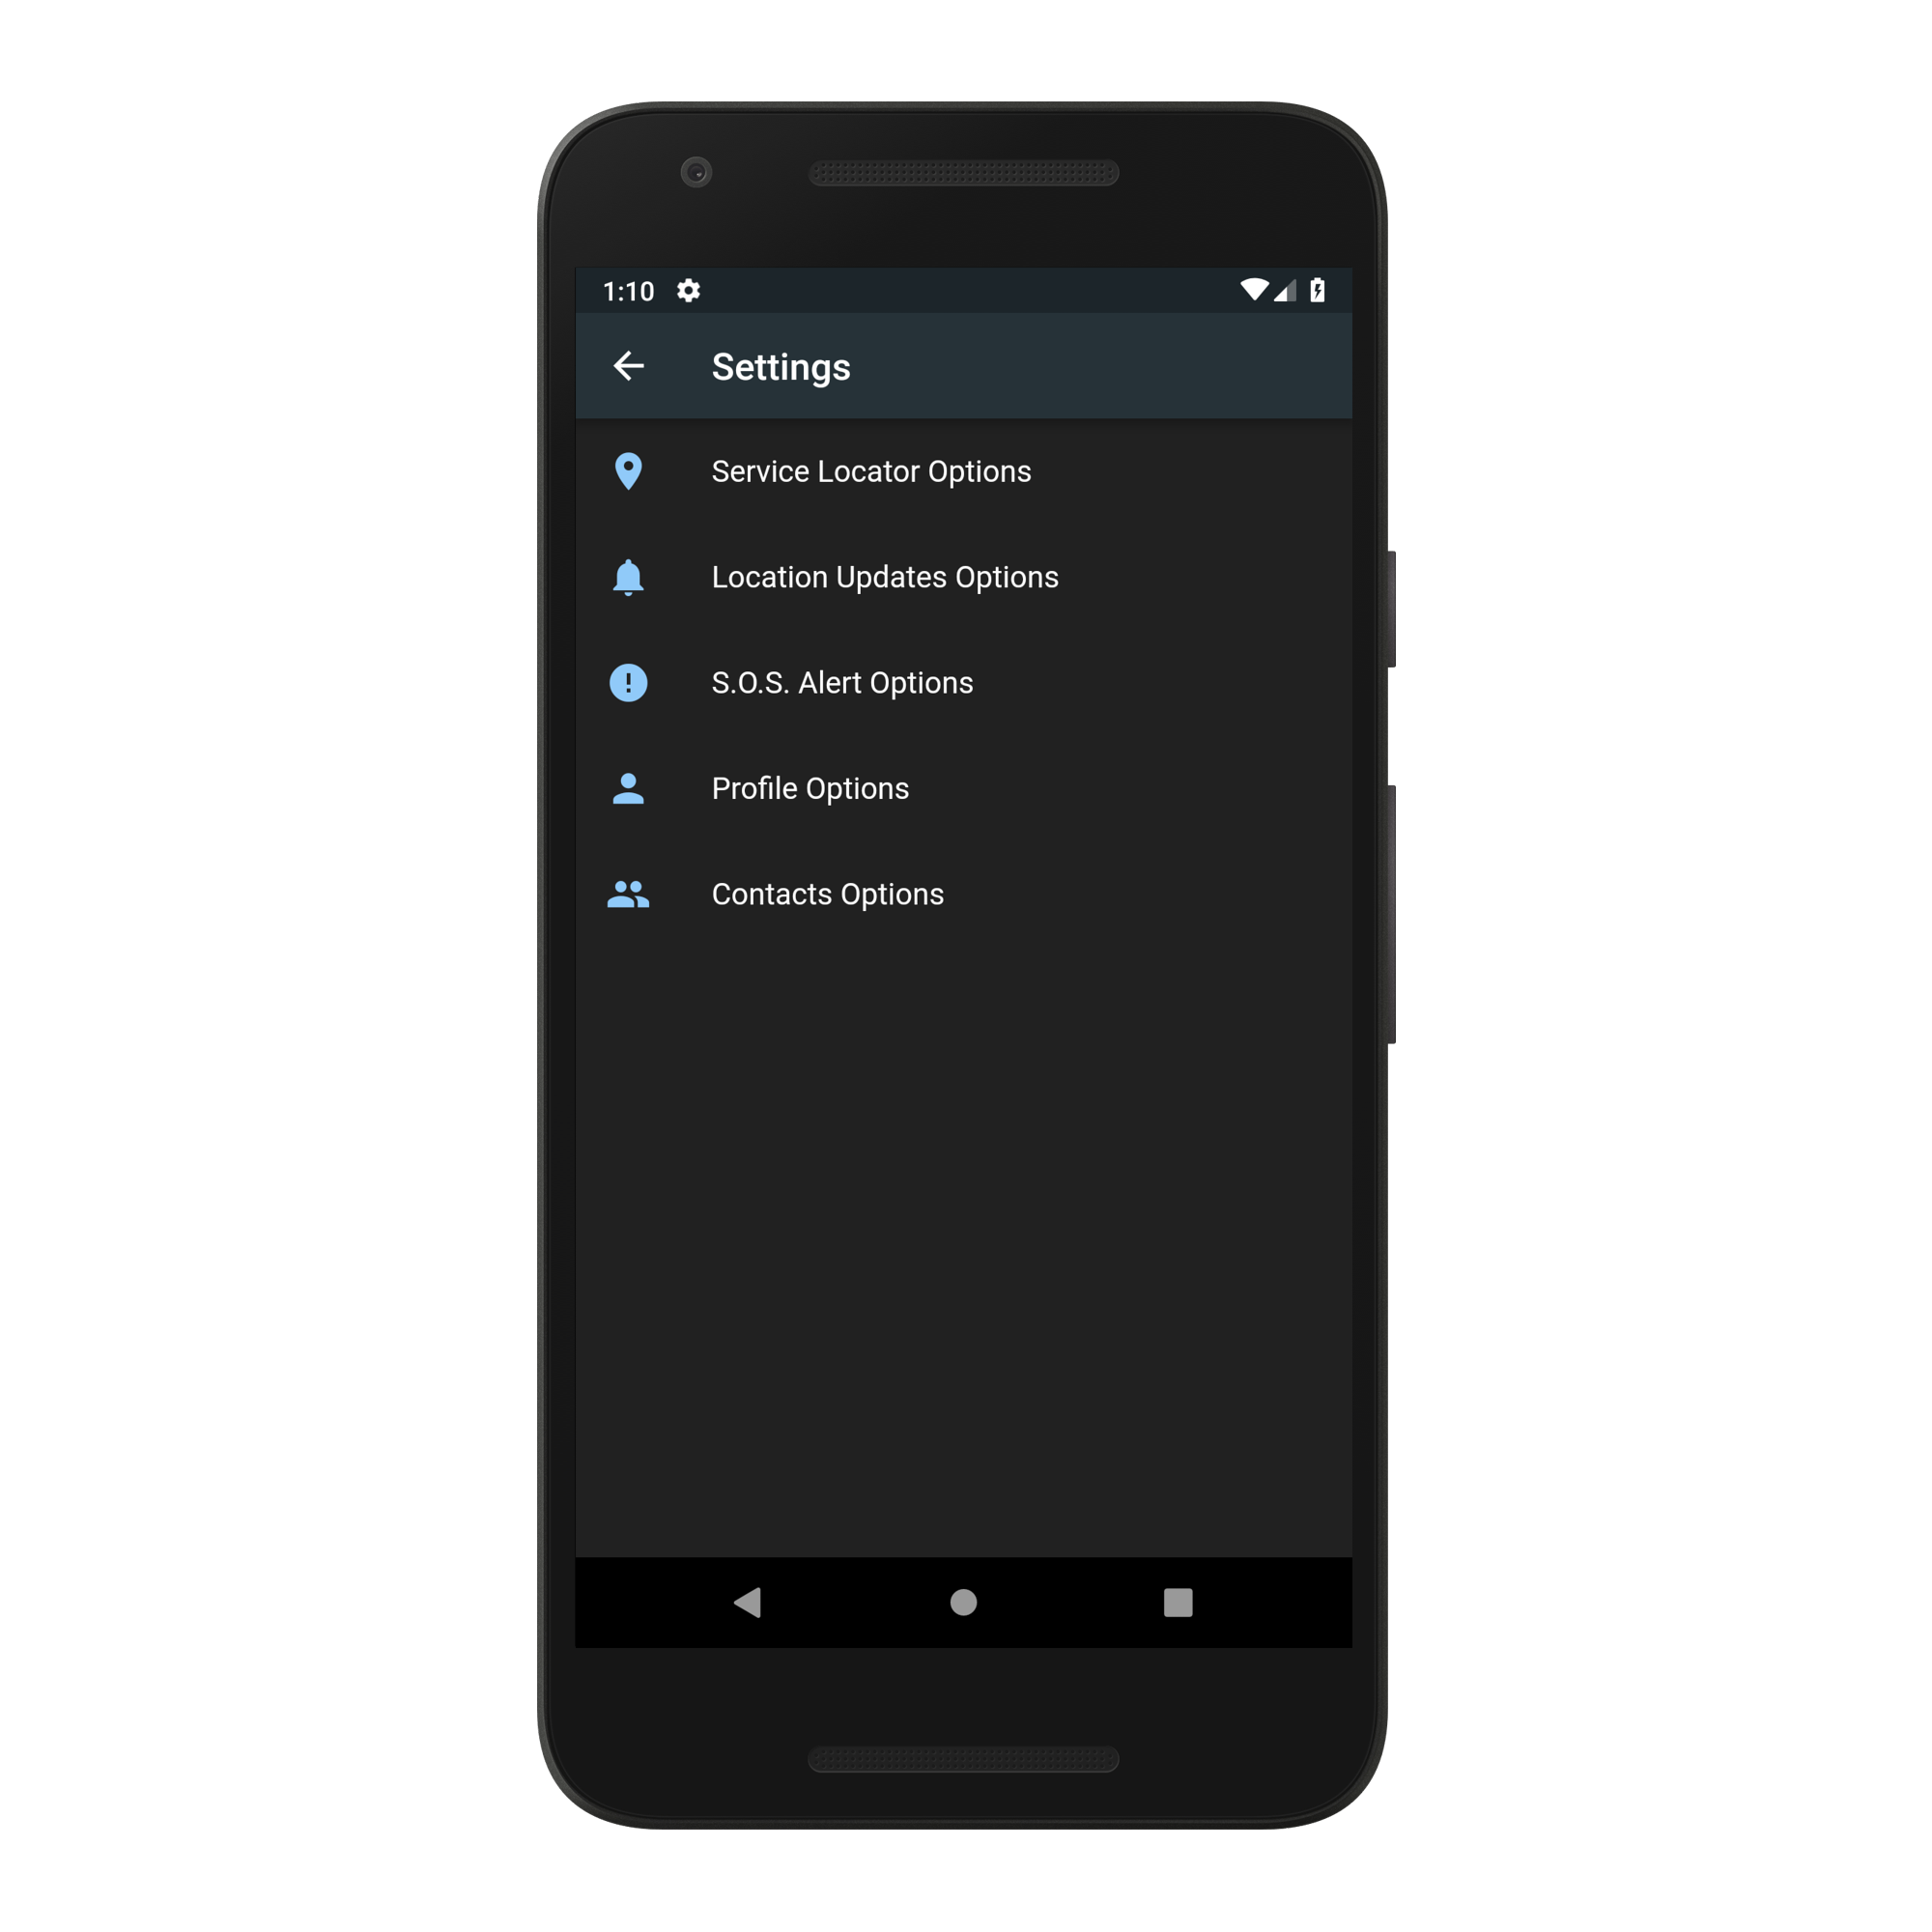
\includegraphics[width=\linewidth]{demo_settings.png}
  \caption{High-fidelity, implemented, screenshot of the mobile client's settings page.}\label{fig:mobile3}
\endminipage
\end{figure}

\begin{figure}[H]
  \centerline{
  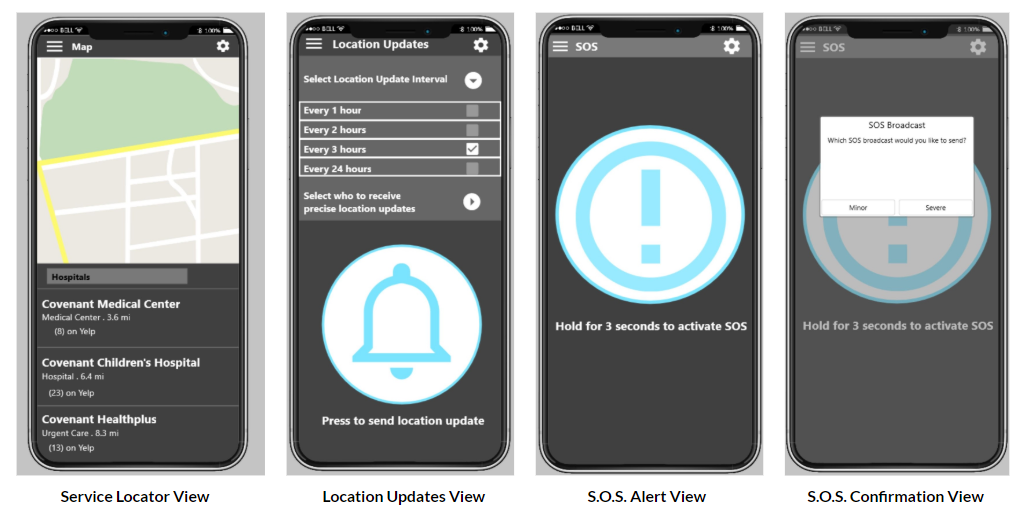
\includegraphics[scale=0.9]{mockups.png}
  }
  \caption{Low-fidelity, mockups of the mobile client's planned service locator, location update, S.O.S. alert and S.O.S. confirmation views. Each of these views would have their own respective widgets as defined in }
\end{figure}

\newpage

\section{Backend Analysis}
\par ~ In this section, we will enumerate the various modules, components, and objects responsible for keeping the backend functional. It should be noted that there is no literal \texttt{class} instance within the Go programming language, but objects may still be enumerated through the \texttt{struct} qualifier. Class attributes are defined as \texttt{struct} fields. Additionally, the backend will follow a decoupled, microservices architecture. Each of these microservices will be defined as a singular, AWS Lambda function which will serve a single purpose.

\begin{figure}[H]
\begin{center}
\centerline{
	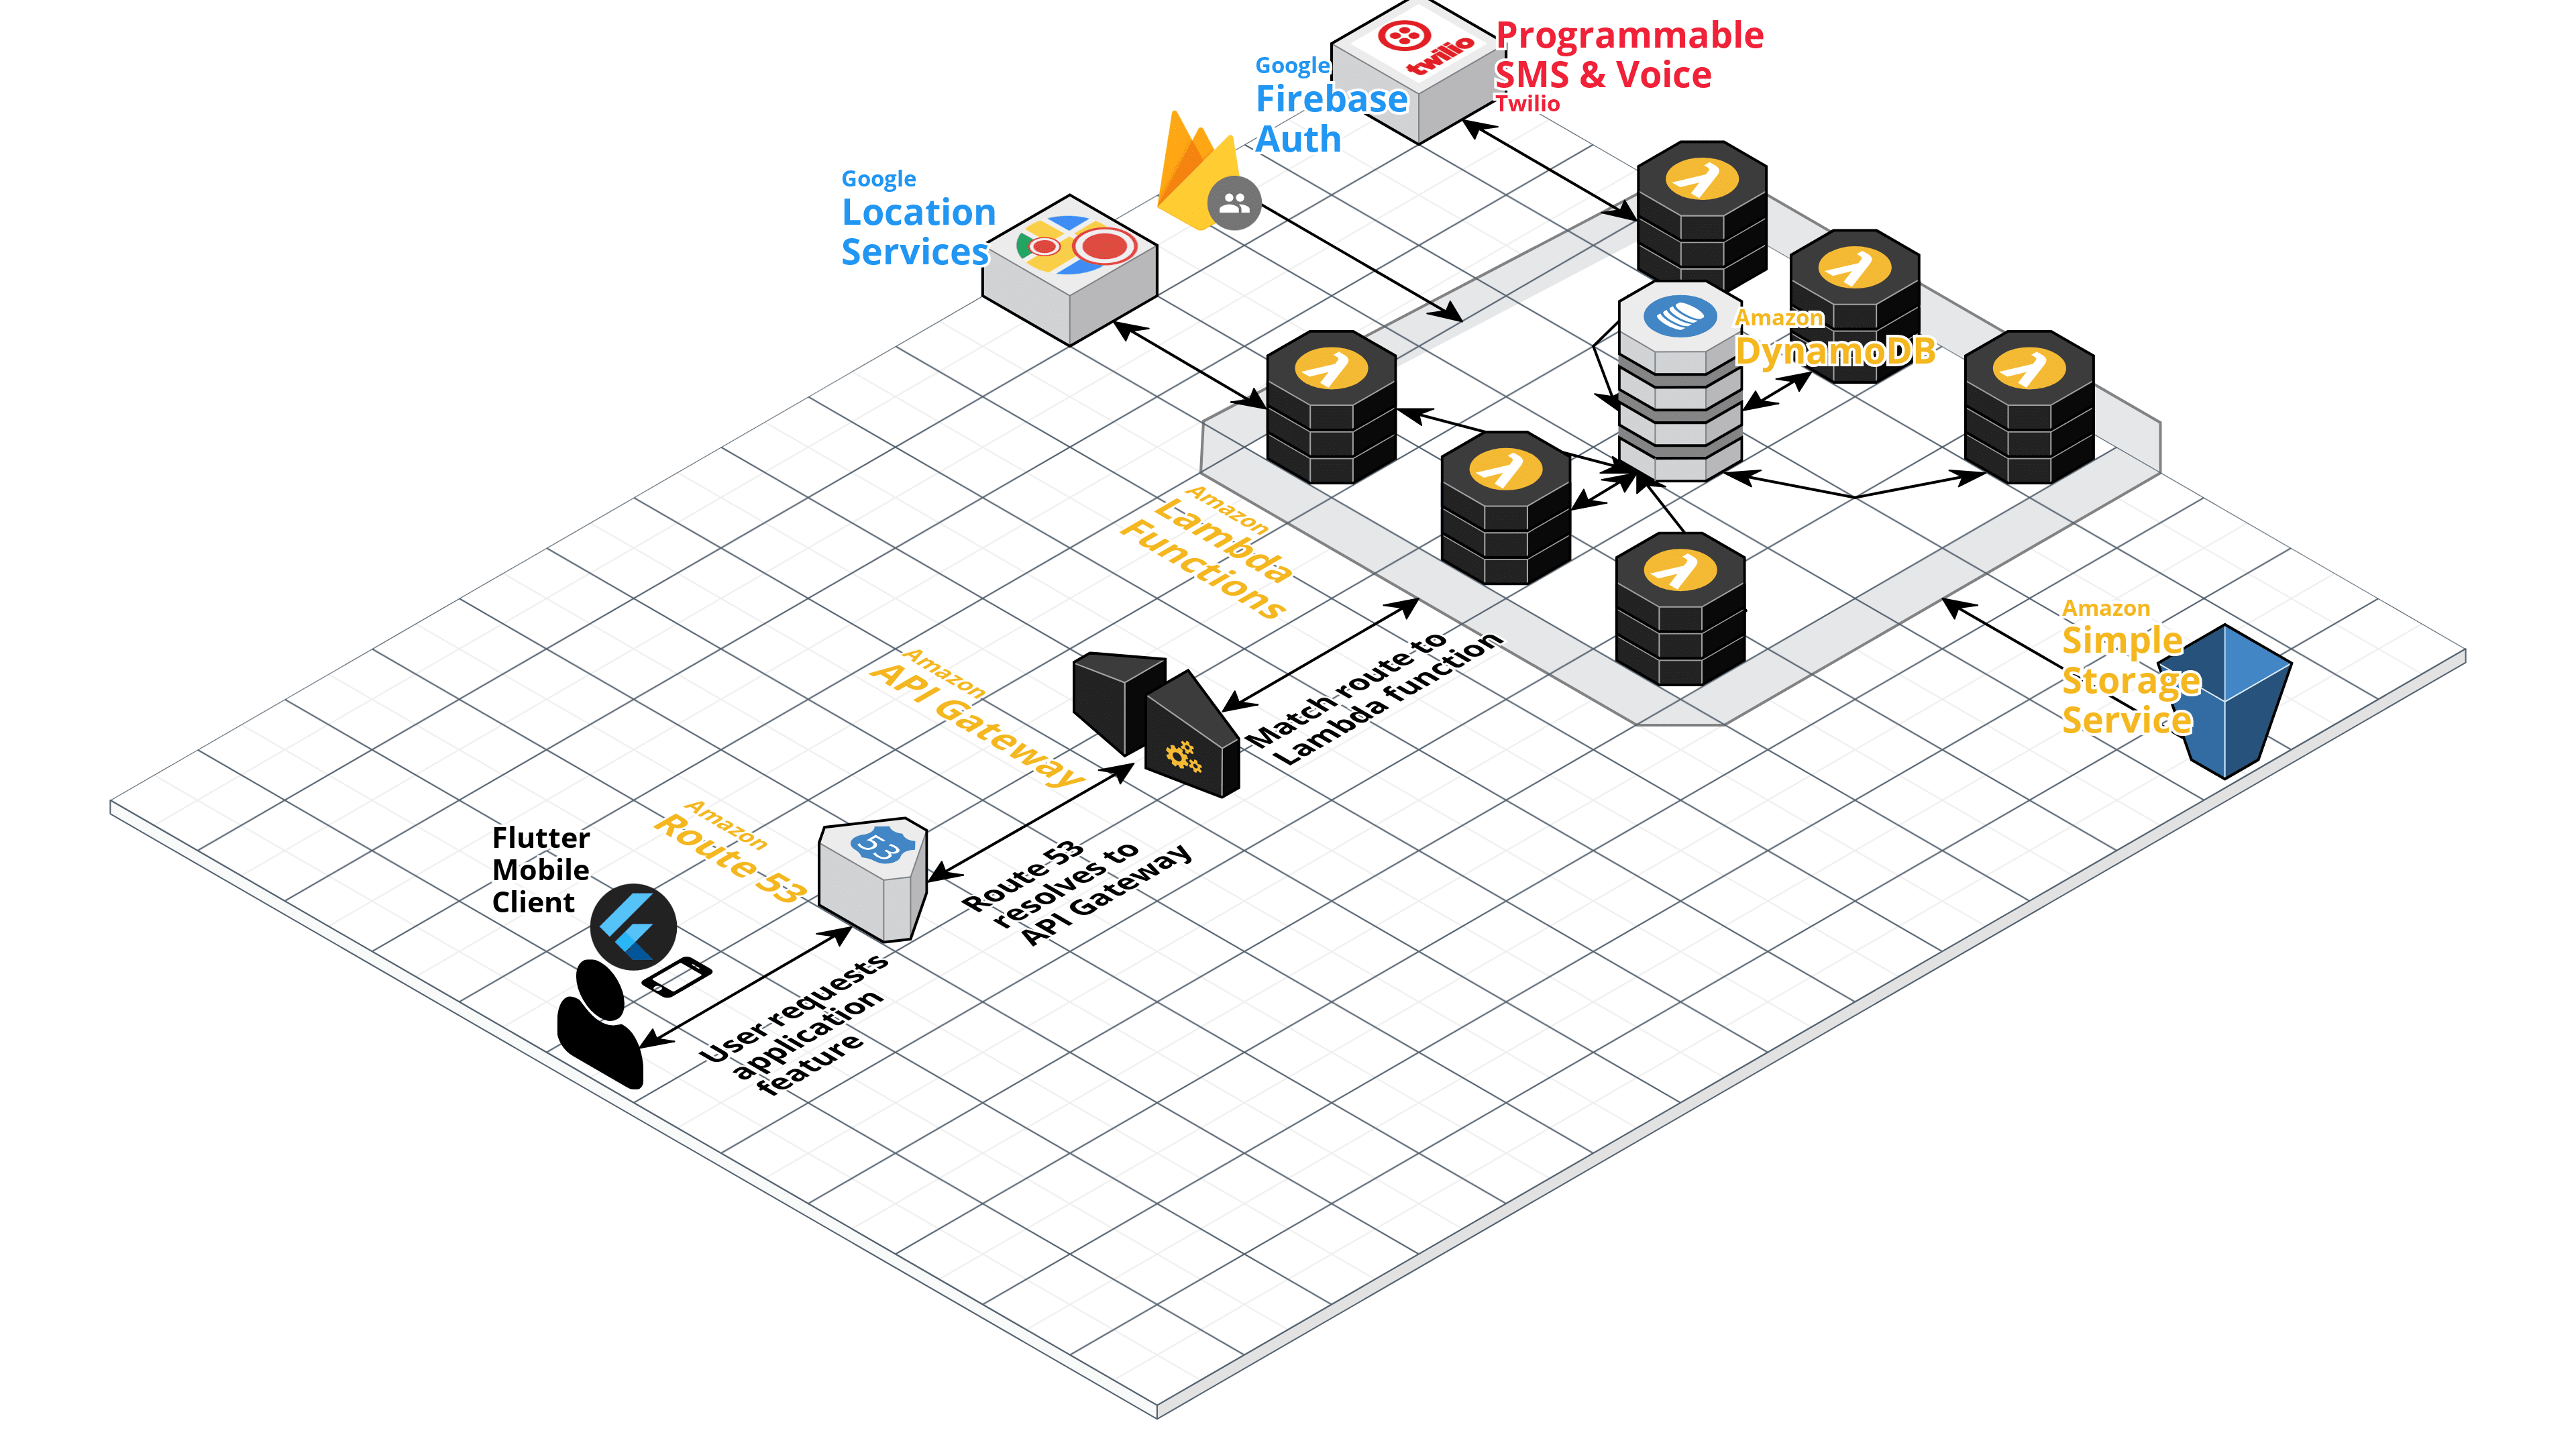
\includegraphics[scale=.15]{EmergenSeek-Backend.PNG}
}
\caption{Cloudcraft \cite{one} diagram of the AWS resources and external APIs necessary for the backend.}
\end{center}	
\end{figure}

\subsection{Models}
\par ~ The models of this application contain Go structures will replicate those defined in the UML Class Diagrams. The functions defined within those models are represented in Go as methods on the \texttt{struct}. For example:

\begin{figure}[H]
	\begin{center}
	\begin{lstlisting}
	type LocationPoller struct {
		// The location to be used for the current poll
		Location  []float32 `json:"location"`
		
		// The user to be used for the current LocationPoller instance
		User      *User     `json:"user"`
		
		// How often the location should be polled	
		Frequency int       `json:"frequency"`
	}

	func (*c LocationPoller) DoSevere() error {
		// Method logic here	
	}
	\end{lstlisting}
	\end{center}
\caption{The code listing above describes how, in Go, a struct is associated with its methods. The method is a pointer receiver on the struct that it is related to. This is similar to how a \texttt{class}, in a language such as Java, has \texttt{class methods}.}
\end{figure}

\subsection{Subsystems}
\par ~ The backend of the application will be comprised of the following. For brevity, each is lambed with a tier:
\begin{enumerate}
	\item[1.] Application Tier - AWS Lambda, a serverless, Functions-as-a-Service offering to run our Go code and AWS API Gateway.
	\item[2.] Database Tier - DynamoDB to store user data and information.
	\item[3.] Notification Tier - The Twilio API to provide the system with programmable SMS and voice communications.
	\item[4.] Location Tier - Google's Geocoding and Maps APIs to better define the location of users and various emergency services.
\end{enumerate}

The subsystems of the application are divided up into single-responsibility, service-oriented architecture. This means that the backend consists of several Lambda functions and each function is responsible for only one thing. In total, at the time of this report, there are \emph{six} Lambda functions. The break down of their functionality and responsibilities are enumerated using a brief description, followed by any additional dependencies that they may have. These dependencies include any external APIs, datastores, or databases. Functions are prefixed with \texttt{ES} and suffixed with a meaningful name which explains their role.

\subsubsection{Lambda Function - ESPollLocation}
\begin{enumerate}
	\item[1.] Function: The purpose of this Lambda function will be to back the location polling feature. The mobile client will run a thread. The thread will sleep until the desired time interval for each notification has passed. When the thread wakes up, it will make a request to this function using the API Gateway endpoint (something like api.emergenseek.com/poll). The request will contain the user's ID and the location of the user at the time that, the thread wakes up. The function will then pull the user from the database, update their last known location, and use Twilio to send granular location information to the user's contacts. The contact ids are stored are foreign objects within the user object that was just retrieved from the database) Note: This function will utilize the Twilio API for communication independently. It will not call the ESSendEmergencySMSMessage Lambda function.
	\item[2.] Dependencies: DynamoDB, Twilio
	\item[3.] HTTP Method: POST
\end{enumerate}
	
\subsubsection{Lambda Function - ESUpdateContactPermissions}
\begin{enumerate}
	\item[1.] Function: The purpose of this Lambda function will be to update the location viewing permissions that  a user's contacts have. For simplicity, a request to this function will include a full User object and the permissions to be set or updated for their contacts.
	\item[2.] Dependencies: DynamoDB, Firebase Auth
	\item[3.] HTTP Method: POST
\end{enumerate}

\subsubsection{Lambda Function - ESSendEmergencySMSMessage}
\begin{enumerate}
	\item[1.] Function: The purpose of this Lambda function will be to send EmergenyType SMS notifications on behalf of a user using Twilio.
	\item[2.] Dependencies: DynamoDB, Twilio
	\item[3.] HTTP Method: POST
\end{enumerate}

\subsubsection{Lambda Function - ESSendEmergencyVoiceCall}
\begin{enumerate}
	\item[1.] Function: The purpose of this Lambda function will be to send EmergencyType programmable voice calls on behalf of a user using Twilio.
	\item[2.] Dependencies: DynamoDB, Twilio
	\item[3.] HTTP Method: POST
\end{enumerate}

\subsubsection{Lambda Function - ESCreateUser}
\begin{enumerate}
	\item[1.] Function: The purpose of this Lambda function will be to create users for the EmergenSeek application
	\item[2.] Dependencies: DynamoDB
	\item[3.] HTTP Method: POST
\end{enumerate}


\subsubsection{Lambda Function - ESGetLockscreenInfo}
\begin{enumerate}
	\item[1.] Function: The purpose of this Lambda function will be to retrieve lock screen information for the user in the event of an emergency. 
	\item[2.] Dependencies: DynamoDB
	\item[3.] HTTP Method: GET
\end{enumerate}

\begin{thebibliography}{9}
\bibitem{one}
Cloudcraft ~ \url{https://cloudcraft.co}
\bibitem{two}
Build Specification Reference for AWS CodeBuild ~ \url{https://docs.aws.amazon.com/codebuild/latest/userguide/build-spec-ref.html}
\bibitem{three}
Testing Flutter apps ~ \url{https://flutter.dev/docs/testing}
\bibitem{four}
Automating Publishing to the Play Store ~ \url{https://github.com/codepath/android_guides/wiki/Automating-Publishing-to-the-Play-Store}
\bibitem{five}
What is the AWS Serverless Application Model (AWS SAM)? ~ \url{https://docs.aws.amazon.com/serverless-application-model/latest/developerguide/what-is-sam.html}
\end{thebibliography}
\end{document}

